\subsection{Winkelhistogramme (Janneke)}
\label{sec:winkelhistogramme}

Um eine Karte anhand von mehreren Laserscans aus unterschiedlichen Positionen aufbauen zu können, müssen diese so ausgerichtet werden, dass sie aneinander passen. Der erste Schritt um dies zu erreichen ist die Rotation, die die Scans zueinander haben, zu berechnen und zu korrigieren. Der erste Schritt zur Berechnung der Rotationskorrektur ist das Erstellen von Winkelhistogrammen für beide Scans.

Das Winkelhistogramm stellt die Winkel der Wände, die aus einem Scan extrahiert werden können, relativ zum Roboter dar. Das Histogramm stellt die Orientierung der Wände in diskreten Schritten von -180 bis +180 Grad dar.

Da wir zunächst in einer Simulation getestet haben, in der wir perfekte Laserscanwerte bekommen, verfolgen wir zunächst einen naiven Ansatz. Hierzu werden je zwei aufeinanderfolgende Scanpunkte betrachtet deren Winkel mit folgender Formel in Radiant berechnet wird: $$angle = atan2(scan[i][1] - scan[i+1][1], scan[i][0] - scan[i+1][0]) * 180 /PI;$$ In Abbildung~\ref{fig:Winkelberechnung} ist der Roboter und eine Wand die dieser mit seinem Laserscanner aufnimmt schematisch dargestellt. An dieser Darstellung wird gezeigt, wie die Formel zur Winkelberechnung zustande kommt.

\begin{figure}
	\centering
	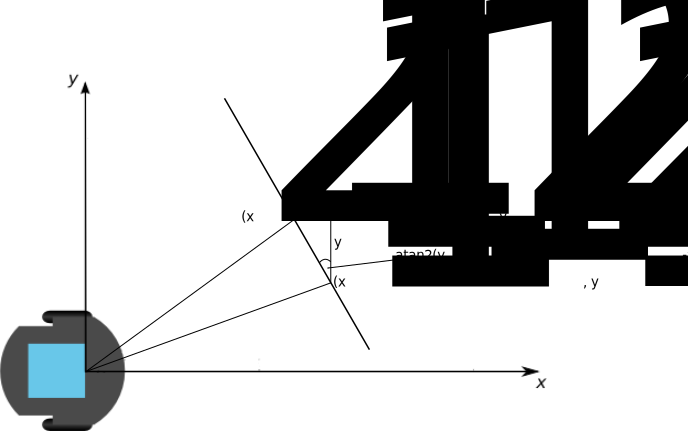
\includegraphics[width=11cm]{atan2}
	\caption{Schema der Berechnung des Winkels zwischen zwei Scanpunkten (Roboter und Koordinatensystem aus der Dokumentation zu scannermap::Scanner)}
	\label{fig:Winkelberechnung}
\end{figure}

Der Winkel den man mit der oben genannten Formel erhält wird in einen entsprechenden Bin im Histogramm umgerechnet, da dieses diskret und nicht kontinuierlich ist. Dazu wurde folgende Formel verwendet, wobei BINCOUNT die Anzahl an Bins im Histogramm ist und damit die Auflösung bestimmt: $$\frac{(angle + 180) * BINCOUNT}{360}$$

Im Histogramm wird dann letztendlich festgehalten, wie oft ein bestimmter Bin (bzw. Winkelbereich) im Scan auftritt. Dadurch werden im Grunde die Wände bzw. geraden Linien die der Laserscanner erfasst dargestellt, da Scanpunkte die auf einer geraden Linie liegen relativ zum Roboter im gleichen Winkel stehen und somit in den gleichen Bin im Histogramm eingeordnet werden. So entstehen im Histogramm Peaks bei den Winkeln, die die Wände relativ zum Roboter haben.

\begin{figure}
	\centering
	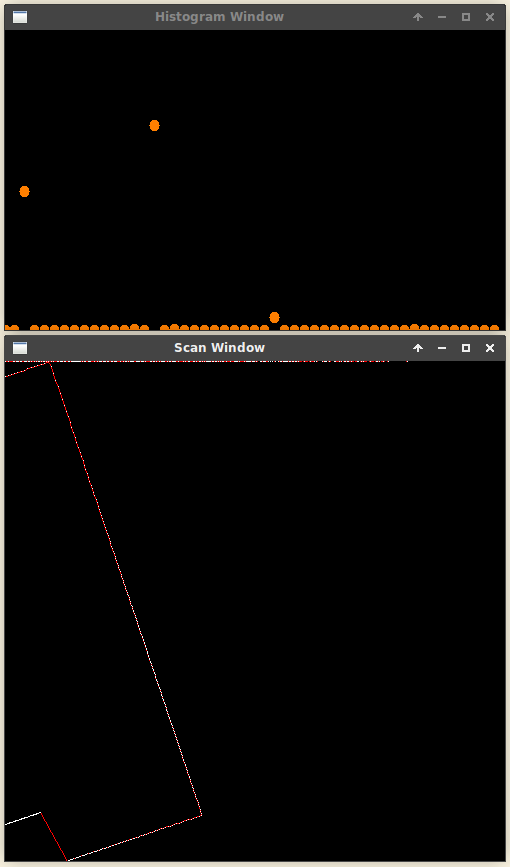
\includegraphics[width=10cm]{winkelhistogramLaserOhneRauschen}
	\caption{Winkelhistogramm (Oben), welches aus dem Laserscan (Unten) berechnet wurde.}
	\label{fig:Winkelhistogramm}
\end{figure}

In Abbildung~\ref{fig:Winkelhistogramm} ist ein Winkelhistogramm, welches wir mit diesem Ansatz erhalten haben, zusammen mit dem Laserscan auf dem es berechnet wurde dargestellt.